

%\documentstyle[epsf,twocolumn]{jarticle}       %LaTeX2.09仕様
%\documentclass[twocolumn]{jarticle}     %pLaTeX2e仕様
\documentclass{jarticle}     %pLaTeX2e仕様

%一枚組だったら[twocolumn]関係のとこ消す

\setlength{\topmargin}{-45pt}
%\setlength{\oddsidemargin}{0cm} 
\setlength{\oddsidemargin}{-7.5mm}
%\setlength{\evensidemargin}{0cm} 
\setlength{\textheight}{24.1cm}
%setlength{\textheight}{25cm} 
\setlength{\textwidth}{17.4cm}
%\setlength{\textwidth}{172mm} 
\setlength{\columnsep}{11mm}

\kanjiskip=.07zw plus.5pt minus.5pt


\usepackage{graphicx}
\usepackage[dvipdfmx]{color}
\usepackage{subcaption}
\usepackage{enumerate}
\usepackage{comment}
\usepackage{url}
\usepackage{multirow}
\usepackage{diagbox}
\usepackage{algorithmic}
\usepackage{amsmath}
\usepackage{algorithm}
\usepackage{lipsum}
\usepackage[jis2004]{otf}
\usepackage{diagbox}


\begin{document}

  \noindent
  \onecolumn
  \hspace{1em}

  \today
  \hfill
  \ \  西村昭賢 

  \vspace{2mm}
  \hrule
  \begin{center}
  {\Large \bf 相談用報告資料}
  \end{center}
  \hrule
  \vspace{3mm}




\section{火曜日からの追加データ}
多目的 GA で勝率に関して優越している解があるかという問いに関して, パレートフロント上の個体の状態しか見ていなかったため再実験した. 図 \ref{fig:nsga2} に結果を示す.

\begin{figure}[htbp]
  \centering
  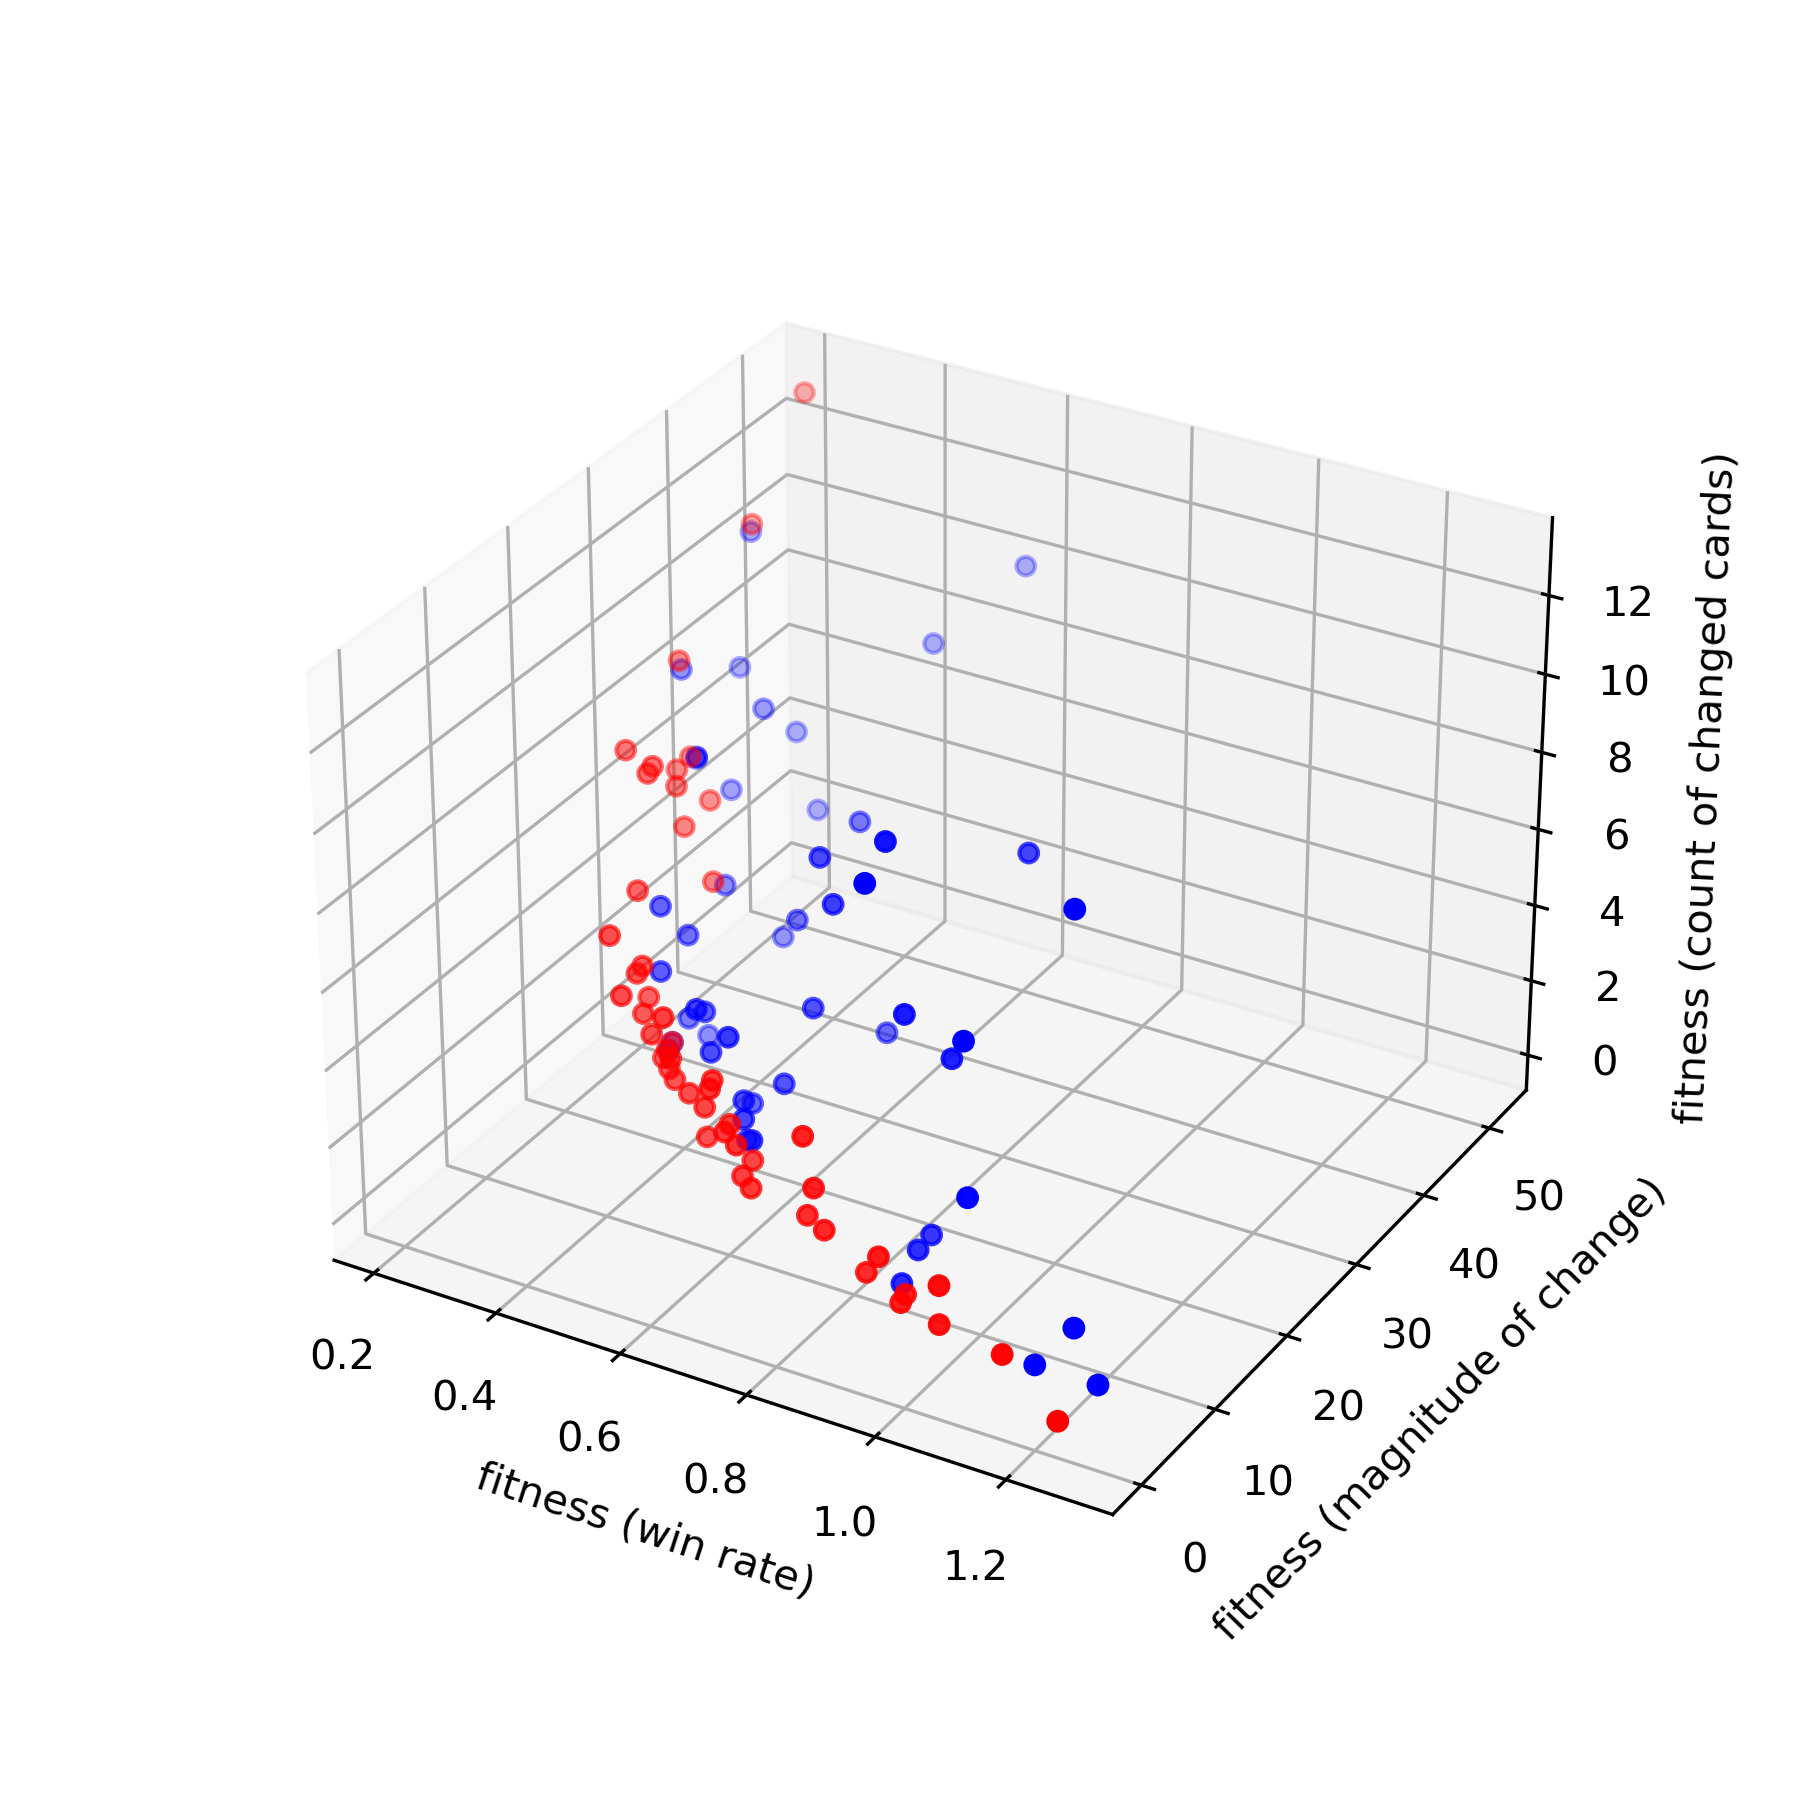
\includegraphics[width=120mm]{assets/nsga2_cardgame.eps}
  \caption{NSGA-II における最終世代の個体 (赤点がパレートフロント, 青点がその他の解)}
  \label{fig:nsga2}
\end{figure}

勝率に着目した場合には, パレートフロント上の勝率最小となる解を選べば良さそう. 
また, 表 \ref{ga_res_2} に再実験した結果の単目的 GA と多目的 GA の比較を示す.

\begin{table}[ht]
  \centering
  \caption{単目的 GA と多目的 GA の比較実験結果}
  \label{ga_res_2}
  \begin{tabular}{|c|c|c|c|}
  \hline
  \diagbox[]{GA}{評価指標}        & パラメータの総変更量 & 勝率に関する適応度 & 変更があったカード枚数 \\ \hline
  単目的 GA      & 80         & \textbf{0.1608}   & 15          \\ \hline
  多目的 GA  & \textbf{41}         & 0.2345   & 13          \\ \hline
  \end{tabular}
  \end{table}

多目的 GA として用いた NSGA-II において遺伝子操作する解の対象は非優越ソートと混雑度ソート上位の個体であるため勝率に関する適応度に関しては, 単目的 GA と比較して同世代同個体数では良い解を発見しづらいと考えられる.

\par
また, 1種類ずつカードをデッキから除いてミラーで対戦させる方法で
$0 > 8 > 6 > 10 > 4 > 1 > 3 > 14 > 2 > 11 > 13 > 9 > 7 > 12 > 5$ の優先順位を作成し高い方からパラメータの変更を認めて徐々に単一 GA の解空間を増やしていく実験をした. 表 \ref{res_now} に結果を示す.

  \begin{table}[ht]
    \centering
    \caption{パラメータ変更するカードを増やしながら単目的 GA を適応した結果}
    \label{res_now}
    \begin{tabular}{|c|c|c|}
    \hline
    変更するカード枚数     & パラメータの総変更量 & 勝率に関する適応度 \\ \hline
    1              & 10         & 0.7330   \\ \hline
    2           & 15         & 0.5288   \\ \hline
    3        & 15         & 0.4893   \\ \hline
    4    & 23         & 0.4559   \\ \hline
    5 & 31         & 0.4471    \\ \hline
    6 & 36      & 0.3962    \\ \hline
    7& 41   & 0.3504    \\ \hline
    8 & 35 & 0.3802  \\ \hline
    9 & 43 & 0.2632 \\ \hline
    10 & 47 & 0.2577 \\ \hline
    11 &  66 & 0.2709 \\ \hline
    12 & 63 & 0.2134 \\ \hline
    13 & 51 & 0.2104 \\ \hline
    
    \end{tabular}
    \end{table}
変更できるカードを増やして, GA の解空間を増やしていけば勝率は減少していった. ただ, 8 枚変更する, 11 枚変更する際には単調減少になっていなかった. 単目的 GA の初期収束が原因だと考えられる. 
カードを 12 枚比較した時の結果に着目し, 表 \ref{ga_res_2} と比較して, 表 \ref{ga_res_3} のように結果を示して優位性的なものが示せたらいいなと考えている. 

\begin{table}[ht]
  \centering
  \caption{GA と NSGA-II の結果}
  \label{ga_res_3}
  \begin{tabular}{|c|c|c|c|}
  \hline
  \diagbox[]{GA}{評価指標}        & パラメータの総変更量 & 勝率に関する適応度 & 変更があったカード枚数 \\ \hline
  単目的 GA      & 80         & \textbf{0.1608}   & 15          \\ \hline
  多目的 GA  & \textbf{41}         & 0.2345   & 13          \\ \hline
  提案手法   & 63               &  0.2134     & \textbf{12}  \\ \hline
  \end{tabular}
  \end{table}
\section{突っ込まれそうな点}
\begin{itemize}
  \item そもそもこの実験は何がしたいのか?
  \par
  先行研究 \cite{DBLP:journals/corr/abs-1907-01623} では多目的 GA である NSGA-2 を用いてデッキ間の勝率をカードのパラメータの変更量を抑えながら最適化していた. しかし, カードのパラメータの変更量を抑えるアプローチは 「アプデなどの状況で一度に大量のカードのパラメータを変更するとユーザーが困惑する」ため考案された. 本研究ではパラメータだけでなくカード自体の変更量も抑えたほうが良いと考えて「変更されるカードの枚数」に注目し, 変更するカードを限定し勝率を最適化する手法を提案する. 本実験は構築環境における提案手法と先行研究の手法との比較の数値実験.
  \item NSGA-2 で勝率と変更カード枚数の 2 つを最適化すれば良いのでは?
  \par
  GA においては交叉や突然変異といった遺伝子操作により変更されるカードを指定できない. バランス調整をするカードを限定して GA により最適化できればうれしいと考えた. (変更するカードを決定 ⇒ パラメータ最適化の流れのほうが自然な気がする)  
  \item アグロ用のデッキとして環境に組み込むならアグロ同士の 1 つ抜きの結果からカードの優先順位作るのが自然じゃない?
  \par
  深層強化学習によるシミュレーションはカードの優先順位もある程度判断するなど人間から見て妥当な戦略を構築している. 最適化したゲーム環境を人間が遊ぶことを想定すると深層強化学習から得た優先順位で調整することが妥当と考えた. (率直には, こうしないと論文としてストーリーがつながらないから)
\end{itemize}

\section{追加で相談したい点}
上記の実験が卒研に入りそうなら, 論文のストーリーとして
\begin{itemize}
  \item 実験 1 : 構築環境への深層強化学習の適用
  \par
  恣意的に強いカード, 弱いカードを 1 種類ずつ入れたデッキを用いる. 
  結果として高い勝率を残すエージェントを作成した. 無駄なターンエンドを減らす, 相手の HP を積極的に減らす, カードの強弱を認識するなど人間から見て妥当な戦略を構築していることが分かった.
  \item 実験 2 : 戦略下におけるデッキ内のカードパワーの測定
  \par
  デッキから 1 種類ずつカードを除いて, 同戦略のプレイヤー同士で対戦を実行した. 結果としてルールベースで作成した AI 同士では恣意的に入れたカード 2 種類が最も強いカード, 最も弱いカードとなったが, 学習済エージェント同士では弱いカードは恣意的に入れたカードとは異なるカードが選ばれた. 
  深層強化学習によるシミュレーションに意味があるといえる.
  \item 実験 3 : 新しいデッキを追加する際のカードゲーム環境の最適化
  \par
  デッキ間の勝率が $50 \pm 5 \%$ になることが好ましい. 実験 1 から用いてきたデッキをアグロ用デッキとして環境へ加えて, 深層強化学習により得た結果からデッキのパラメータを調整する. 単目的 GA と比較して少ないパラメータの変更量で, 多目的 GA と比較して少ない変更枚数でより小さい勝率に関する適応度を持つ解 (デッキ) を得ることができ, 勝率に関して最適化されたトレーディングカードゲーム環境を構築できた. 
\end{itemize}
といった感じで構成しようと考えている. 

また, 提案手法としては 「深層強化学習によるデッキの最適な戦略の構築とその戦略下におけるそれぞれのカードパワーの測定」, 「解空間を限定した GA による TCG 環境の最適化」になると考えている. 

%index.bibはtexファイルと同階層に置く
%ちゃんと\citeしないと表示されない(1敗)
\bibliography{index.bib}
\bibliographystyle{junsrt}

\end{document}